\chapter{Redes Neuronales Bayesianas en RISC-V}

En esta sección se explican los pasos y bibliotecas desarrolladas para poder ejecutar inferencia de BNN de manera eficiente en un procesador RISC-V con solo soporte para precisión entera. La Figura \ref{fig:experiment_pipeline} muestra el proceso y componentes necesarios.

\begin{figure}[h]
    \centering
    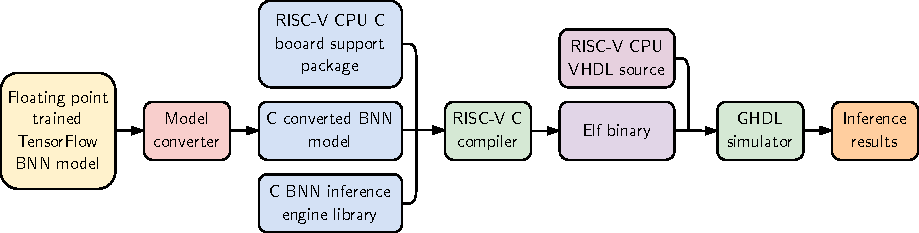
\includegraphics[width=\textwidth]{Imagenes/experiment_pipeline.pdf}
    \caption{\todo}
    \label{fig:experiment_pipeline}
\end{figure}

\section{Componentes desarrollados}

Para poder llevar a cabo el proceso de la Figura \ref{fig:experiment_pipeline} se han realizado las siguientes tareas: desarrollar un conversor de modelos, desarrollar un motor de inferencia de BNN, actualizar el \textit{\textbf{B}oard \textbf{S}upport \textbf{P}ackage} (BSP) del procesador y desarrollar una herramienta de análisis de resultados.

\subsection{Conversor de modelos}

Se ha desarrollado una herramienta en Python que convierte modelos BNN TensorFlow ya entrenados en precisión de punto flotante a ficheros de código C que puedan ejecutarse junto al motor de inferencia explicado en la Sección \ref{sec:motor_inferencia_c}. Esta herramienta realiza las siguientes tareas:

\begin{itemize}
    \item Transformar los pesos a coma fija. Coma fija es un formato que permite representar y operar con números decimales utilizando hardware de precisión entera.
    \item Analizar la precisión mínima necesaria. Buscar el tamaño de dato más pequeño en los que los pesos transformados se puedan almacenar. \todo
    \item Generar vectores de pesos. Generar código C que almacene los pesos en vectores aplanados.
    \item Generar función de inferencia. Analizar que capas forman el modelo y generar el código de una función de inferencia utilizando las funciones proveídas por el motor.
    \item Transformar los datos de prueba a coma fija.
    \item Generar vector de datos de prueba.
\end{itemize}

\subsection{Actualización del Board Support Package}

Con el objetivo de mejorar la experiencia de desarrollo del motor de inferencia se actualizó el BSP del procesador para dar soporte a la biblioteca estándar C (libc) y algunas funcionalidades de C++. De esta forma se pueden utilizar funciones útiles de libc cómo \texttt{printf}, o \texttt{memset} entre otras. Para ello se actualizaron las herramientas y ficheros de compilación, se añadieron funciones \textit{stub} para las llamadas al sistema no implementadas y se implementaron versiones modificadas de \texttt{\_write} y \texttt{\_exit}.

\subsection{Motor de inferencia} \label{sec:motor_inferencia_c}

Se ha desarrollado una librería de funciones que ejecutan la inferencia de capas BNN estándar y convolucionales con funciones de activación ReLU o exponenciales normalizadas (SoftMax) utilizando precisión de punto fijo. Mientras que calcular la función ReLU es trivial la función SoftMax no. Dicha función toma un vector de componentes $x \in X$ de tamaño $N$ como entrada y devuelve otro del mismo tamaño cuyos componentes $y\in Y$ se calculan según la Ecuación \ref{eq:softmax}.
\begin{equation} \label{eq:softmax}
y_i = \dfrac{e^{x_i}}{\sum_{j = 0}^N e^{x_j}}
\end{equation}

Para calcular esta función utilizando coma fija es necesario calcular la función exponencial en dicho formato. Para evitar desbordamientos de la función exponencial se va a utilizar la función SoftMax equivalente mostrada en la Ecuación \ref{eq:softmax_neg}.
\begin{equation} \label{eq:softmax_neg}
y_i = \dfrac{e^{x_i - \max(X)}}{\sum_{j = 0}^N e^{x_j - \max(X)}}
\end{equation}

En esta versión de la función se cumple que $x_i \in (-\infty, 0]$ por lo que $e^{x_i} \in (0,1]$. Para calcular la función exponencial se va a utilizar la Ecuación \ref{eq:split_exp}, dividiendo la entrada $x_i$ en su parte entera $a_i$ y su parte decimal $b_i$.
\begin{equation} \label{eq:split_exp}
e^{x_i} = e^{a_i+b_i} = e^{a_i} e^{b_i}
\end{equation}

La parte entera $e^{a_i}$ se calcula mediante una LUT de 20 entradas para el rango $[e^{-19}, e^{0}]$. A partir de $e^{-19}$ los valores son demasiado pequeños como para representarlos con la precisión disponible por lo que siempre valen $0$. La parte decimal $e^{b_i}$ se aproxima mediante los 8 primeros términos de la serie de Taylor mostrada en la Ecuación \ref{eq:exp_taylor}. Para optimizar y evitar las divisiones los valores de $\dfrac{1}{n!}$ para $n \in [2,7]$ se han almacenado en una LUT.
\begin{equation} \label{eq:exp_taylor}
e^{b_i} \approx \sum_{n=0}^{7} \dfrac{{b_i}^n}{n!}
\end{equation}

Como se ha explicado previamente, las BNN necesitan muestrear distribuciones gaussianas. Como método de muestreo base se utilizada un algoritmo basado en la suma de distribuciones uniformes, dicha suma se aproximan a una distribución gaussiana debido al TCL, mostrado en la Ecuación \ref{eq:tcl_unif}.
\begin{equation} \label{eq:tcl_unif}
\sum_{n=0}^{N} \mathcal{U}_n(0,1) \sim \mathcal{N} \left( \dfrac{N}{2}, \sqrt{\dfrac{N}{12}} \right)
\end{equation}

El algoritmo implementado genera muestras de $\mathcal{N}(0,1)$ para luego transformarlas en muestras de una distribución gaussiana arbitraria $\mathcal{N}(\mu, \sigma)$ de media $\mu$ y desviación típica $\sigma$ utilizando la Ecuación \ref{eq:gauss_linear}.
\begin{equation} \label{eq:gauss_linear}
\mathcal{N}(\mu, \sigma) = \sigma \mathcal{N}(0,1) + \mu
\end{equation}

Para ello utiliza la suma de 12 distribuciones uniformes y posteriormente centra la distribución como muestra la Ecuación \ref{eq:tcl_12center}.
\begin{equation} \label{eq:tcl_12center}
\sum_{n=0}^{12} \mathcal{U}_n(0,1) - 6 \sim \mathcal{N}(0,1)
\end{equation}

Para generar muestras de distribuciones uniformes se utiliza una versión del algoritmo Xorshift de 32 bits \cite{xorshift}. Es un algoritmo sencillo para generar números pseudoaleatorios solamente con instrucciones \texttt{xor} y \texttt{shift}.

Para calcular las métricas de incertidumbre se necesita la función logaritmo por lo que se ha implementado una versión del algoritmo desarrollado por Turner \cite{binary_log} para calcular el logaritmo de un número en coma fija. 

\subsection{Verificación automática}

Para analizar el correcto funcionamiento del motor de inferencia y estudiar el impacto en el rendimiento de las optimizaciones posteriores se ha desarrollado una herramienta que compara las predicciones del conjunto de datos de prueba obtenidas con el motor de inferencia y TensorFlow.

Para comparar los conjuntos de predicciones se han utilizado la métrica de precisión y las métricas de incertidumbre. La precisión es simplemente el ratio de predicciones correctas sobre el número de predicciones. Analizar las métricas de incertidumbre es más complejo, por lo que se han utilizado los siguientes gráficos para ello.\\



\boxtext{
\begin{itemize}
    \item \todo
    \item incertidumbre media de cada clase
    \item histograma de las predicciones correctas, incorrectas
    \item recta calibración
    \item precisión por grupos
    \item cambio de prueba
    \item cambio de prueba B
    \item cambios hechos desde el mundo local despues del merge
\end{itemize}
}

\section{Análisis de la carga de trabajo}



\section{Optimizaciones software}

